\section{Monte Carlo Simulation of Synthetic Data}

% Discussion of how observed points were measured and located
\noindent
Before beginning with the implementation of the Monte Carlo simulation, it is pertinent to explain the sampling procedure as  it took place in the field.  These points will be referred to as the \textit{observed} points henceforth.  From site to site, 4-10 observed points were measured each day, with some sites having more than 4-10 observed points when measurements were repeated (e.g. GVNT).  

% Defining sample spaces and distribution of observed points
\vspace{3mm} \par \noindent
For this study, sample spaces are defined by ways: 1) by name and 2) geographically.  A sitename (e.g. EETR, GVNT, MMTH) defines the name of a sample space. Geographically, sample spaces were defined from images drawn from Google Earth Pro. After the observed points were uploaded to Google Earth Pro, an image capturing the points and the surrounding area (30-50 meters in each direction from the center of of observed points) was downloaded and used as the sample space.  Figure 1 highlight an example of the sample space at PRCN is defined geographically.

\begin{figure}[h]
    \centering
    \subfigure[]
    {
        \label{fig:first}
        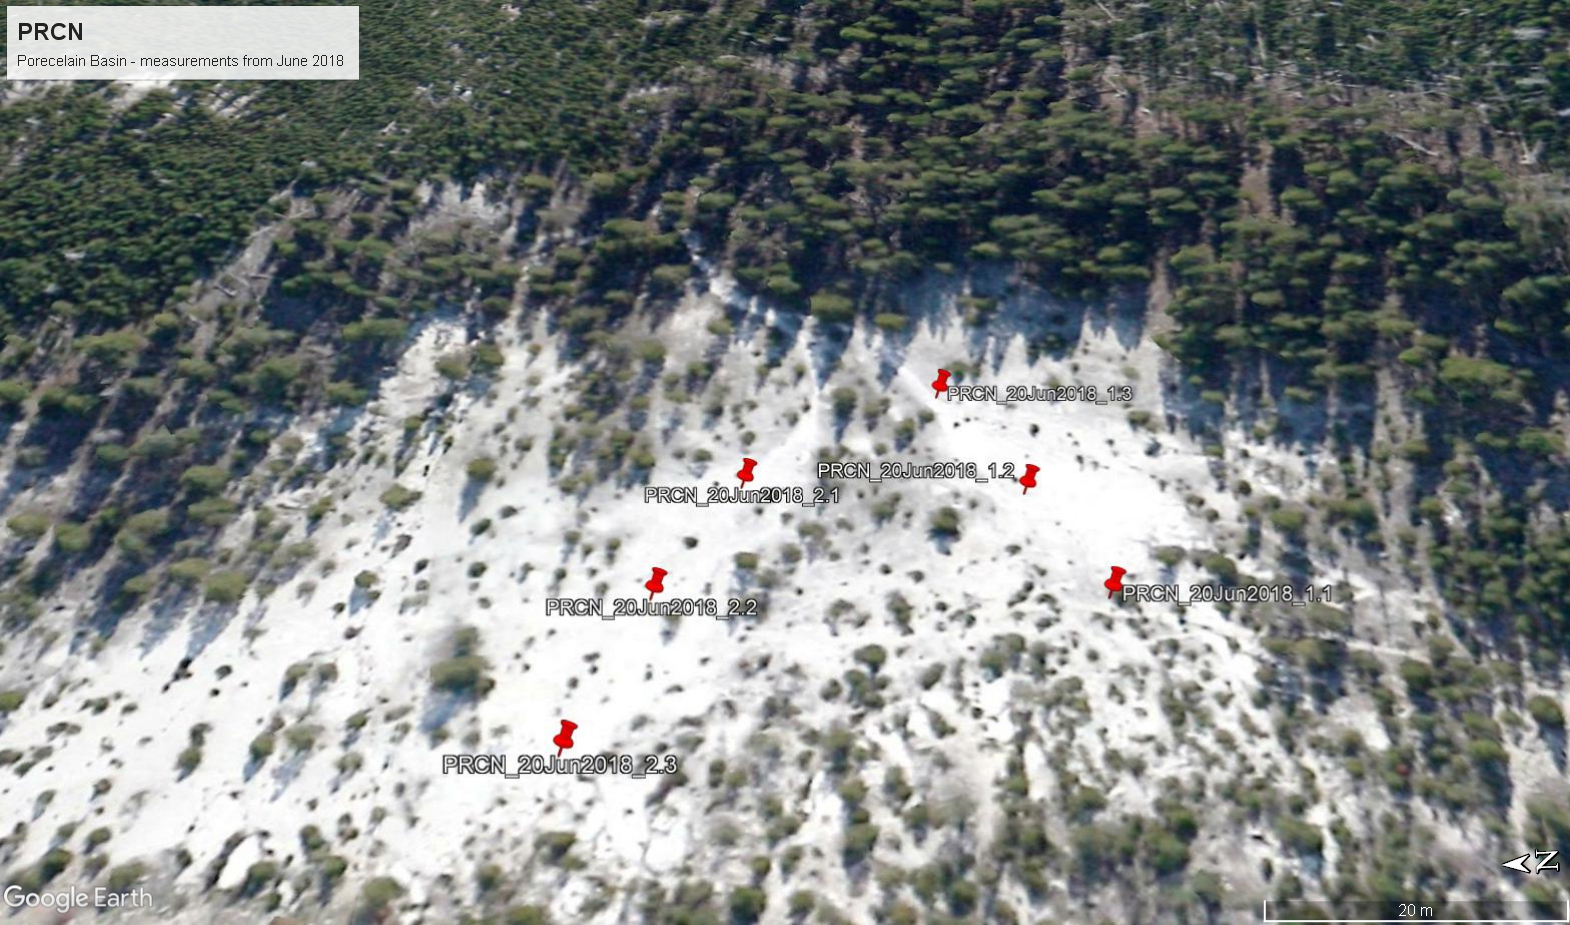
\includegraphics[width=0.6\textwidth]{Figures/PRCN_2018_Sampling_Locations.jpg}
    }
    \subfigure[]
    {
        \label{fig:second}
        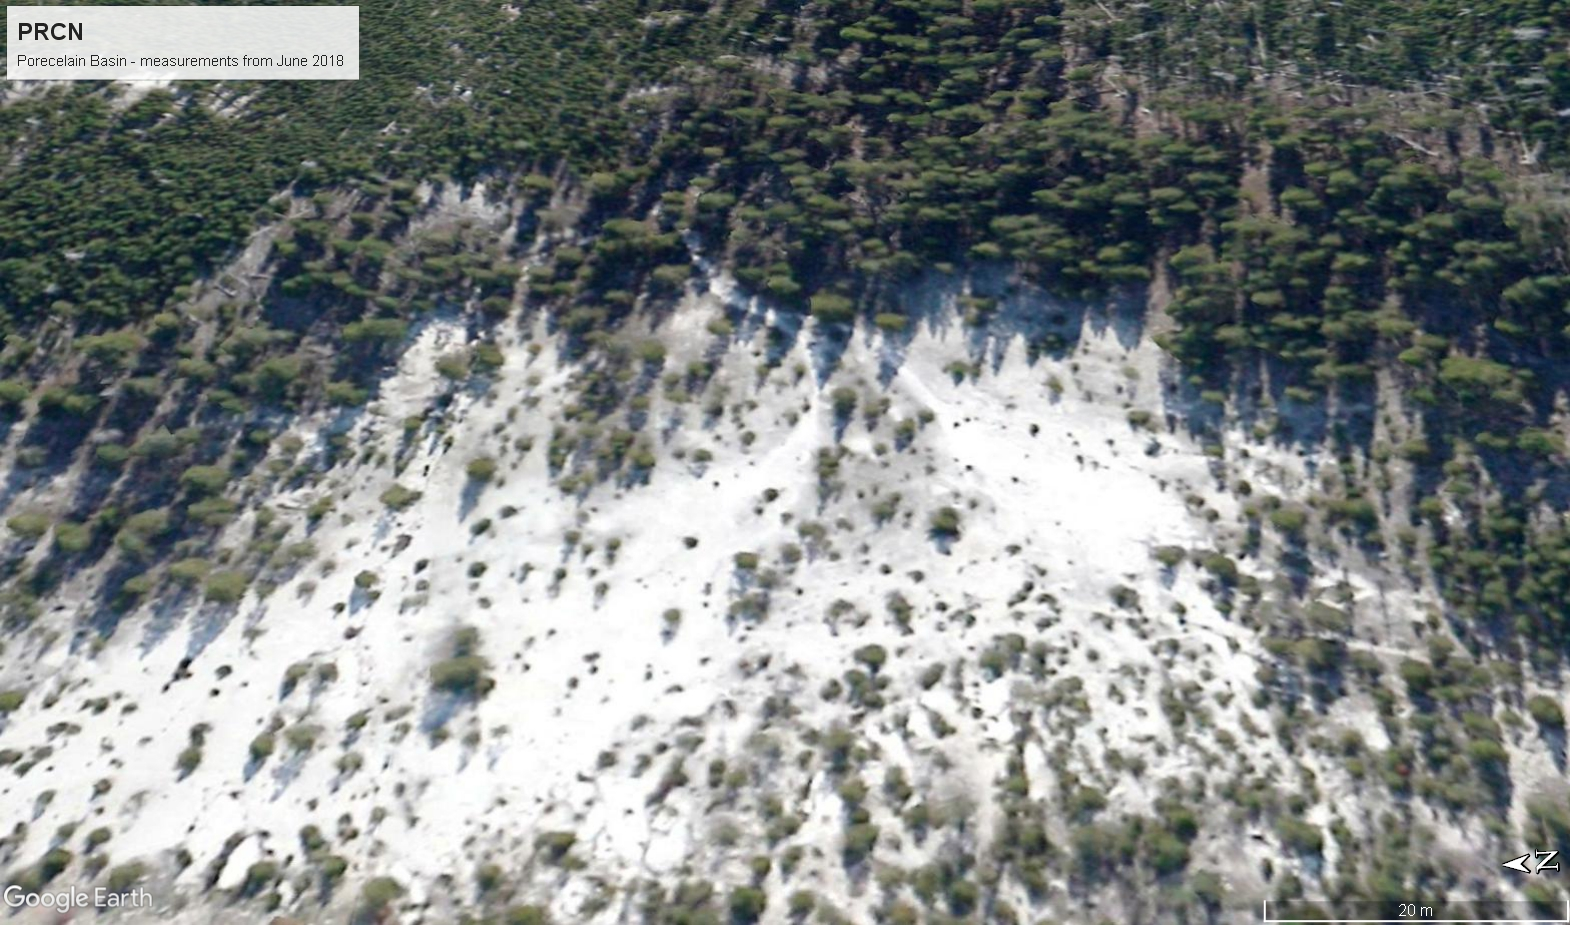
\includegraphics[width=0.6\textwidth]{Figures/PRCN_2018_Sampling_Locations_no_LABELS.jpg}
    }
    \caption{Sampling spaces at PRCN, shown with (a) and without (b) the location of the observed points}
    \label{fig:subfigures}
\end{figure}

% Distribution of observed points
\vspace{3mm} \par \noindent
With the sample space defined, the distribution of observed points was analyzed to assess. Let sample space be defined by $\Omega$ and the observed points as $\X$.  For PRCN, we divided the image into a six part grid (2 x 3). The distribution of observed points was then analyzed and categorized as random, regular, or clustered (McKillup and Dyar 2010).  Figure 2 illustrates the grid and the observed points.  Using a Poisson distribution, the expected number of observation points per grid space was calculated based on the assumption of a regular spread, or one point per grid space.  This assumption, the population mean ($\mu$) and the observed points per grid space are entered into the following equation:

\begin{equation}
    \label{eq1}
    P(X) = \frac{e^{-\mu} \mu^{X}}{X!}
\end{equation}

\noindent
When $P(X)$ is less than or equal to 0.05, the distribution was labelled significantly non-random.  By anlayzing the variance ($s^{2}$) to sample mean ratio ($\overline{X}$), the determination of a non-random distribution of observed points can be labelled as regular if $s^{2}$:$\overline{X} < 1$ and clustered if $s^{2}$:$\overline{X} > 1$.  

\begin{figure}
    \centering
    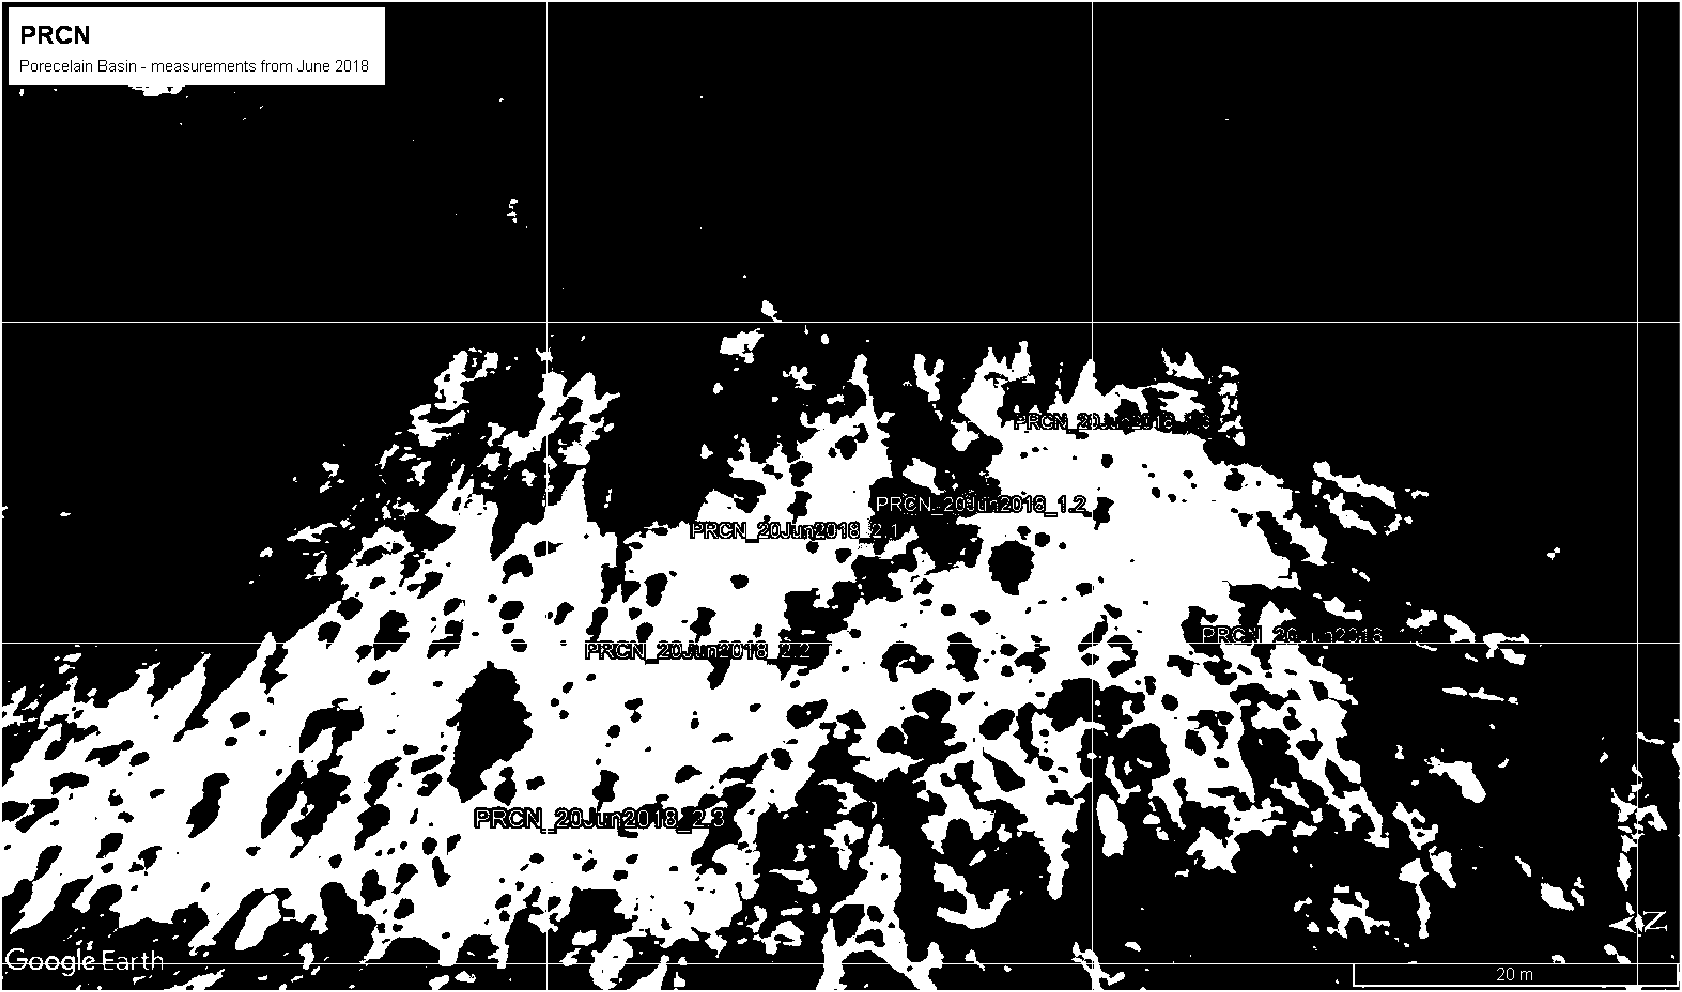
\includegraphics[scale=0.8,width=0.8\textwidth]{Figures/PRCN_3x3_BW.png}
    \caption{PRCN sample space in binary (black versus white) and with observation points present.  This gridded image was used to determine the distribution of observed points in the sample space.}
    \label{fig:my_label}
\end{figure}

% Implementing the synthetic dataset